\section*{Задание 3}
    Разложить в ряд Фурье функцию \( f(x) = \cos x - e^x \) по системе собственных функций \( \{ 1, \cos(\varphi n x), \sin(\varphi n x) \}, n = 1,\dots,\infty \) задачи Штурма-Лиувилля.

    Ряд Фурье имеет вид 
    \[
        f(x) = A_0 + \sum_{n=1}^{\infty} \left( A_n \cos(nx) + B_n \sin(nx) \right).
    \]

    Найдём коэффициенты:
    \[
        A_0 = \frac{1}{2\pi} \int_{0}^{2\pi} f(x) dx = \frac{1}{2\pi} \int_{0}^{2\pi} \left( \cos x - e^x \right) dx = \frac{1}{2\pi} \left( \sin x - e^x \right) \big|_0^{2\pi} = \frac{1 - e^{2\pi}}{2\pi},
    \]

    \[
        A_n = \frac{1}{\pi} \int_{0}^{2\pi} f(x) \cos(nx) dx = \frac{1}{\pi} \int_{0}^{2\pi} \left( \cos x - e^x \right) \cos(nx) dx =
    \]
    \[
        = \frac{1}{\pi} \left( \frac{n \sin(2\pi n)}{n^2 - 1} + \frac{1 - e^{2\pi} \left( n \sin(2\pi n) + \cos(2\pi n)\right)}{n^2+1}\right) = \frac{1 - e^{2\pi}}{\pi (n^2 + 1)}, n > 1.
    \]
    \[
        A_1 = \frac{1}{\pi} \int_{0}^{2\pi} \left( \cos x - e^x \right) \cos(x) dx = \frac{1}{\pi} \left( \pi + \frac{1 - e^{2\pi}}{2} \right)= 1 + \frac{1 - e^{2\pi}}{2\pi}
    \]

    \[
        B_n = \frac{1}{\pi} \int_{0}^{2\pi} f(x) \sin(nx) dx = \frac{1}{\pi} \int_{0}^{2\pi} \left( \cos x - e^x \right) \sin(nx) dx =
    \]
    \[
        = \frac{1}{\pi} \left( \frac{2n \sin^2(2\pi n)}{n^2 - 1} + \frac{e^{2\pi} \left(n \cos(2\pi n) - \sin(2\pi n)\right) - n}{n^2+1}\right) = \frac{n\left(e^{2\pi} - 1\right)}{\pi (n^2 + 1)}, n > 1.
    \]
    \[
        B_1 = \frac{1}{\pi} \int_{0}^{2\pi} \left( \cos x - e^x \right) \sin(x) dx = \frac{1}{\pi} \left( \frac{e^{2\pi} - 1}{2} \right) = \frac{e^{2\pi} - 1}{2\pi}
    \]

    \begin{figure}[H]
        \centering
        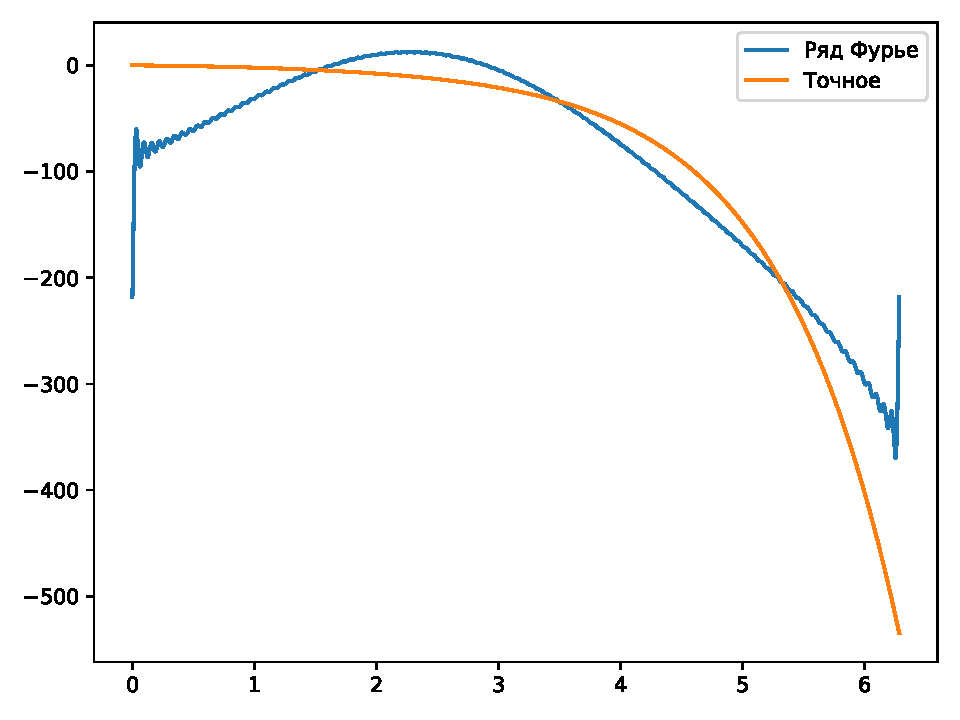
\includegraphics[width=14cm]{fur1.pdf}
        \caption{При \( n = 100 \).}
    \end{figure}

    Разложим на интервале \( [-\pi, \pi] \).
    \[
        A_0 = \frac{1}{2\pi} \int_{-\pi}^{\pi} f(x) dx = \frac{e^{-\pi} - e^{\pi}}{2\pi},
    \]

    \[
        A_n = \frac{1}{\pi} \int_{-\pi}^{\pi} f(x) \cos(nx) dx = \frac{1}{\pi} \int_{-\pi}^{\pi} \left( \cos x - e^x \right) \cos(nx) dx =
    \]
    \[
        = \frac{1}{\pi} \left( -\frac{2 n \sin(\pi n)}{n^2 - 1} - 2 \frac{\sinh(\pi) \cos(\pi n) + n \cosh(\pi) \sin(\pi n)}{n^2+1}\right) = \frac{2 \sinh(\pi) (-1)^{n+1}}{\pi (n^2 + 1)}, n > 1.
    \]
    \[
        A_1 = \frac{1}{\pi} \int_{-\pi}^{\pi} \left( \cos x - e^x \right) \cos(x) dx = 1 + \frac{\sinh(\pi)}{\pi}
    \]

    \[
        B_n = \frac{1}{\pi} \int_{-\pi}^{\pi} f(x) \sin(nx) dx = \frac{1}{\pi} \int_{-\pi}^{\pi} \left( \cos x - e^x \right) \sin(nx) dx =
    \]
    \[
        = \frac{1}{\pi} 2 \frac{n \sinh(\pi) \cos(\pi n) - \cosh(\pi) \sin(\pi n)}{n^2 + 1} = \frac{2 n \sinh(\pi) (-1)^n}{\pi(n^2 + 1)}.
    \]

    \begin{figure}[H]
        \centering
        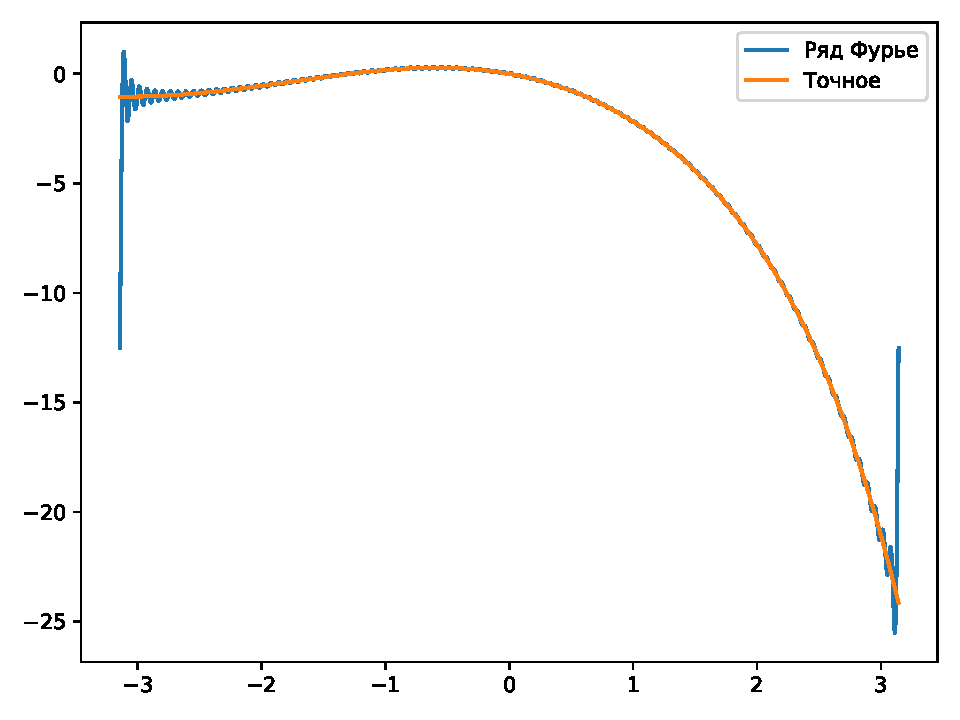
\includegraphics[width=14cm]{fur2.pdf}
        \caption{При \( n = 100 \).}
    \end{figure}